\chapter {Anexo I: Manual Usuario}
	\section{Despliegue automático sobre bare metal}
		\subsection{Requisitos previos}
			\subsubsection{Hetzner}
				\begin{paragraph}
					Para el alquiler de infraestructura hemos confiado en Hetzner. Para el completo funcionamiento de este proyecto, es necesario tener contratados servidores bare metal en Hetzner. 
						\begin{itemize}
							\item Ip adicional nodos maestros.
							\item MAC adicional para ip adicional nodos maestros.
							\item IP failover. Contratar failover ip en uno de los nodos maestros.
							\item Virtual Switch conexión nodos en cluster. Conectar todos los nodos al VSwtich.
							\item Clave pública. Fingerprint. Agregar fingerprint a la interfaz de Hetzner.
						\end{itemize}	
					Todo lo anterior se puede encontrar cómo hacerlo en los manuales de Hetzner \cite{hetznerdocs:online}
				\end{paragraph}
			\subsubsection{Dominio}
				\begin{paragraph}
					Contratar un dominio en cualquier proveedor o utilizar uno ya existente. En esta sección vamos a utilizar los siguientes dominios:
					\begin{itemize}
						\item nodo1.dominio.com
						\item nodo2.dominio.com 
						\item nodo3.dominio.com
						\item pfsense-01.dominio.com
						\item pfsense-02.dominio.com
						\item failover.dominio.com
					\end{itemize}
				\end{paragraph}
			\subsubsection{Clonar repositorio desde Github}
				\begin{paragraph}
					En primer lugar, debemos clonar el repositorio en la máquina que vaya a ejecutar los playbooks. Esto es muy sencillo el único requisito es tener git instalado:
					
					\lstset{language=Bash}
					\begin{lstlisting}
						git clone git@github.com:VictorMorenoJimenez/tfg2020.git
					\end{lstlisting}
					 
				\end{paragraph}
			\subsubsection{Ansible Hosts}
				\begin{paragraph}
					Una vez clonado el proyecto, tendremos la siguiente estructura de carpetas:
					\lstset{language=Bash}
					\begin{lstlisting}
						ansible
							ansible.cfg
							inventories
							Makefile
							playbooks
							roles
						doc
							images
							latex
							playbooks
							README.md
							role
						LICENSE
						Makefile
						README.md
						scripts
							create-ansible-folder-structure.sh
							create-new-roles.sh  
					\end{lstlisting}
					
					Antes de comenzar debemos definir nuestros hosts bajo el directorio inventories. Que fichero de host se utiliza se define en el Makefile. En el fichero hosts.yml debemos definir los nombres que vamos a utilizar para referenciar a los hosts dentro de los playbooks, debemos configurar las IP y las variables de cada host. Un ejemplo del fichero hosts.yml:
					\clearpage 
					
					\lstset{language=xml}
					\begin{lstlisting}
					---
					all:
			 			hosts:
				  			children:
							proxmox_master:
								hosts:
									tfg.intelligenia.com:
									ansible_host: tfg.intelligenia.com  
									ansible_user: root
									node: tfg
							proxmox_slave:
								hosts:
									tfg2.intelligenia.com:
									ansible_host: tfg2.intelligenia.com 
									ansible_user: root
									node: tfg2
							proxmox_nodes:
								hosts:
									tfg3.intelligenia.com:
									ansible_host: tfg3.intelligenia.com 
									ansible_user: root
									node: tf3
							proxmox:
								hosts:
									tfg.intelligenia.com:
									tfg2.intelligenia.com:
									tfg3.intelligenia.com:
							
							pfsense_master:
								hosts:
									pfsense-01.tfg.vps:
									ansible_host: 138.201.229.85
									ansible_user: root  
							pfsense_slave:
								hosts:
									pfsense-02.tfg.vps:
									ansible_host: 144.76.2.118
									ansible_user: root  
							pfsense:
								hosts:
									pfsense-01.tfg.vps:
									pfsense-02.tfg.vps:
					\end{lstlisting}
					
				\end{paragraph}
			\subsubsection{Dependencias. Configuración host}
				\begin{paragraph}
					Los playbooks los podemos lanzar desde nuestro equipo local o un host remoto donde clonemos el repositorio. Para ejecutar los playbooks y utilizar todos los módulos de Ansible, necesitamos instalar algunas dependencias. A continuación se listan dichas dependencias:
					\begin{itemize}
						\item Ansible 2.9.11
						\item Python 3.7
						\item Proxmoxer pip
						\item requests pip 
						\item Molecule
						\item Docker
					\end{itemize}
				\end{paragraph}
			
			
		\subsection{Activación Rescue Hetzner}
			\begin{paragraph}
				Otro de los requisitos para comenzar a ejecutar los playbooks de Ansible es tener activado el modo rescate en los servidores Hetzner. En el panel de configuración de Hetzner, podemos activar el modo rescate.A continuación se muestra un ejemplo:
					\begin{figure}[!hbt]
						\centering
						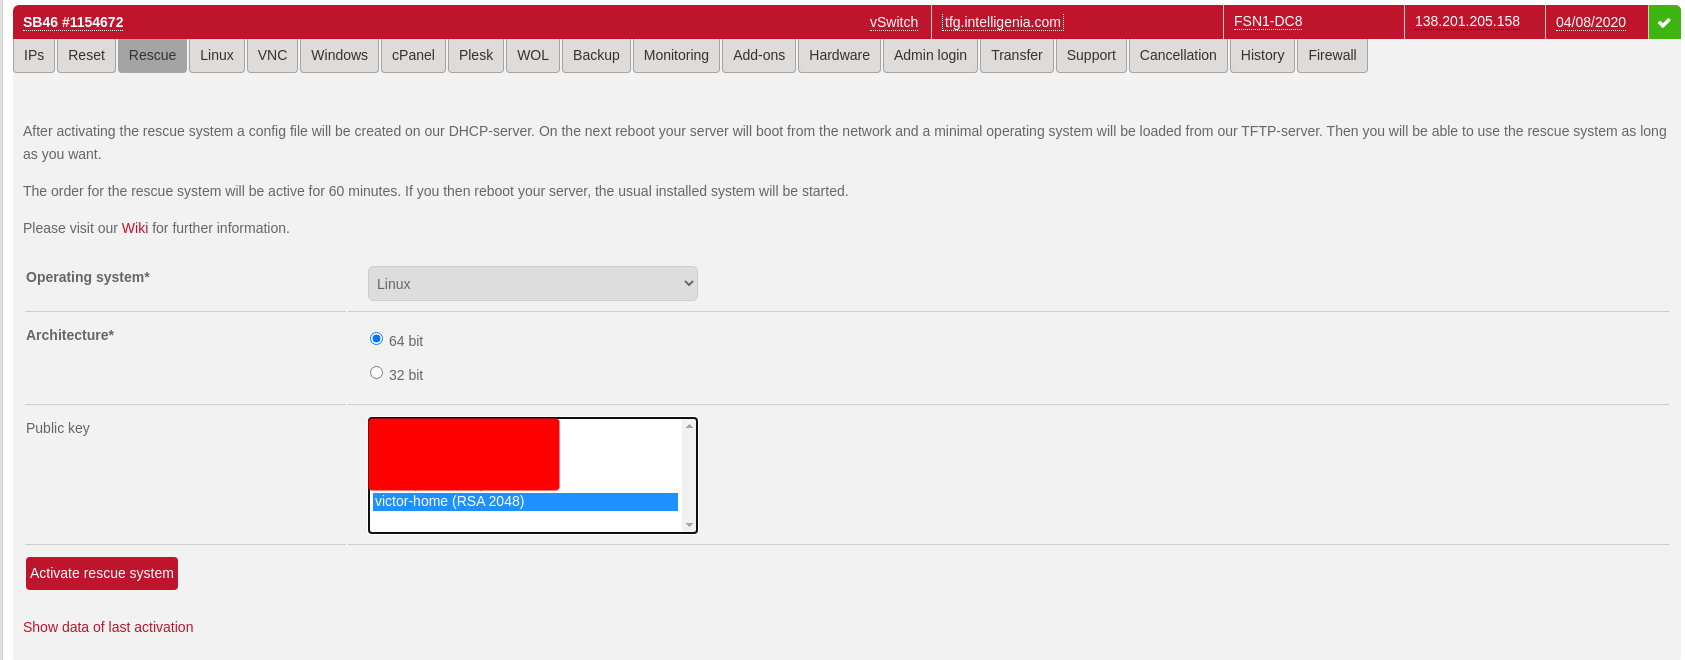
\includegraphics[scale=0.27]{imagenes/Manual/activar_rescue.png}
						\caption[ActivateRescue]{ActivateRescue}
						\label{ActivateRescue}
					\end{figure}
			\end{paragraph}
		\subsection{Configuración variables Playbook}
		\begin{paragraph}
			Para la configuración de los nodos proxmox disponemos del playbook playbook/configure\_proxmox\_node.yml.
			En la sección inicial del playbook, hay ciertas variables que se pueden configurar. En el propio playbook están explicadas las variables.
			\begin{itemize}
				\item \textbf{partitions}: Particiones a definir. 
				\item \textbf{logical\_volumes}: Volúmenes logicos, no cambiar el nombre del grupo de volúmenes.
				\item \textbf{iso}: Imagen para instalar en el modo rescate de Hetzner.
				\item \textbf{configure\_node\_opt}: Configuración del nodo.
				\item \textbf{configure\_users\_goups\_opt}: Agregar usuarios y grupos de bash al nodo.
				\item \textbf{install\_proxmox\_opt}: Instalar proxmox en los nodos.
				\item \textbf{configure\_storages\_opt}: Instalar distintos almacenamientos en proxmox.
				\item \textbf{configure\_ssl\_letsencrypt\_opt}: Instalar certificado SSL con letsencrypt.
				\item \textbf{create\_proxmox\_users\_opt}: Crear usuarios proxmox.
				\item \textbf{create\_proxmox\_groups\_opt}: Crear grupos proxmox.
				\item \textbf{vlan\_nodes\_id}: VSwitch vlan para los nodos proxmox
				\item \textbf{vlan\_lan\_id}: VSwitch vlan para lan.
				\item \textbf{vlan\_pfsync\_id}: VSwitch vlan para pfSync.
				\item \textbf{vlan\_nodes2\_id}: VSwitch vlan redundante para nodos proxmox.
				\item \textbf{servername}: Dominio del nodo.
				\item \textbf{certbot\_admin\_email}: Admin email para la instalación de certificado ssl.
				\item \textbf{create\_ssl\_certificate\_opt}: Opción para instalar certificado ssl o no. Debe ser yes para que se instale.
			\end{itemize}
	
			Aditional vars can be found on Hetzner role vars.yml file.
		\end{paragraph}
		\subsection{Ejecución Playbook}
			\begin{paragraph}
				Para la ejecución del playbook nos situamos bajo la carpeta ansible. Disponemos de un Makefile para invocar los distintos playbooks. En nuestro caso:
				\lstset{language=bash}
				\begin{lstlisting}
					make PLAYBOOK=configure_proxmox_node TAGS=all HOST=proxmox playbook
				\end{lstlisting}
			\end{paragraph}
		\clearpage
		Si todo va bien el playbook debe finalizar con una salida exitosa. Nótese que algunas tareas se saltan debido a que terminan con error, pero si son saltadas on "skipped" no afectan al correcto funcionamiento, lo podemos ignorar. A continuación se muestra un ejemplo de la correcta ejecución del playbook. (Este playbook tarda alrededor de 15 minutos en ejecutarse.)
		
		\begin{figure}[!hbt]
			\centering
			\includegraphics[scale=0.27]{imagenes/Manual/ejecucion_playbook1.png}
			\caption[Ejecucion1]{Ejecucion1}
			\label{Ejecucion Configure proxmox nodes}
		\end{figure}
		
	\section{Despliegue automático y aprovisionamiento de máquinas virtuales}
		\begin{paragraph}
			Tras la finalización del playbook anterior, ya tenemos los 3 nodos configurados con Proxmox instalado y el cluster iniciado. Partimos de la siguiente configuración:
			
			\begin{figure}[!hbt]
				\centering
				\includegraphics[scale=0.27]{imagenes/Manual/proxmoxcluster.png}
				\caption[Proxmox cluster]{Proxmox cluster}
				\label{Proxmox_cluster}
			\end{figure}
		
			A partir de aquí se explica como desplegar cada uno de los distintos servicios del cluster. 			
		\end{paragraph}
		\subsection{pfSense}
		\subsection{GitLab}
			\subsubsection{GitLab Runner}
		\subsection{Webproxy}
		\subsection{Docker Swarm}
		\subsection{Kubernetes}
		\subsection{Galera cluster}
		\subsection{Ceph}
		\subsection{RabbitMQ}
		\subsection{Virtualmin}
		